% Options for packages loaded elsewhere
\PassOptionsToPackage{unicode}{hyperref}
\PassOptionsToPackage{hyphens}{url}
%
\documentclass[
  10pt,
  letterpaper,
  DIV=11,
  numbers=noendperiod,
  twoside]{scrartcl}

\usepackage{amsmath,amssymb}
\usepackage{setspace}
\usepackage{iftex}
\ifPDFTeX
  \usepackage[T1]{fontenc}
  \usepackage[utf8]{inputenc}
  \usepackage{textcomp} % provide euro and other symbols
\else % if luatex or xetex
  \usepackage{unicode-math}
  \defaultfontfeatures{Scale=MatchLowercase}
  \defaultfontfeatures[\rmfamily]{Ligatures=TeX,Scale=1}
\fi
\usepackage{lmodern}
\ifPDFTeX\else  
    % xetex/luatex font selection
  \setmainfont[ItalicFont=EB Garamond Italic,BoldFont=EB Garamond
Bold]{EB Garamond Math}
  \setsansfont[]{Europa-Bold}
  \setmathfont[]{Garamond-Math}
\fi
% Use upquote if available, for straight quotes in verbatim environments
\IfFileExists{upquote.sty}{\usepackage{upquote}}{}
\IfFileExists{microtype.sty}{% use microtype if available
  \usepackage[]{microtype}
  \UseMicrotypeSet[protrusion]{basicmath} % disable protrusion for tt fonts
}{}
\usepackage{xcolor}
\usepackage[left=1in, right=1in, top=0.8in, bottom=0.8in,
paperheight=9.5in, paperwidth=6.5in, includemp=TRUE, marginparwidth=0in,
marginparsep=0in]{geometry}
\setlength{\emergencystretch}{3em} % prevent overfull lines
\setcounter{secnumdepth}{3}
% Make \paragraph and \subparagraph free-standing
\ifx\paragraph\undefined\else
  \let\oldparagraph\paragraph
  \renewcommand{\paragraph}[1]{\oldparagraph{#1}\mbox{}}
\fi
\ifx\subparagraph\undefined\else
  \let\oldsubparagraph\subparagraph
  \renewcommand{\subparagraph}[1]{\oldsubparagraph{#1}\mbox{}}
\fi


\providecommand{\tightlist}{%
  \setlength{\itemsep}{0pt}\setlength{\parskip}{0pt}}\usepackage{longtable,booktabs,array}
\usepackage{calc} % for calculating minipage widths
% Correct order of tables after \paragraph or \subparagraph
\usepackage{etoolbox}
\makeatletter
\patchcmd\longtable{\par}{\if@noskipsec\mbox{}\fi\par}{}{}
\makeatother
% Allow footnotes in longtable head/foot
\IfFileExists{footnotehyper.sty}{\usepackage{footnotehyper}}{\usepackage{footnote}}
\makesavenoteenv{longtable}
\usepackage{graphicx}
\makeatletter
\def\maxwidth{\ifdim\Gin@nat@width>\linewidth\linewidth\else\Gin@nat@width\fi}
\def\maxheight{\ifdim\Gin@nat@height>\textheight\textheight\else\Gin@nat@height\fi}
\makeatother
% Scale images if necessary, so that they will not overflow the page
% margins by default, and it is still possible to overwrite the defaults
% using explicit options in \includegraphics[width, height, ...]{}
\setkeys{Gin}{width=\maxwidth,height=\maxheight,keepaspectratio}
% Set default figure placement to htbp
\makeatletter
\def\fps@figure{htbp}
\makeatother
% definitions for citeproc citations
\NewDocumentCommand\citeproctext{}{}
\NewDocumentCommand\citeproc{mm}{%
  \begingroup\def\citeproctext{#2}\cite{#1}\endgroup}
\makeatletter
 % allow citations to break across lines
 \let\@cite@ofmt\@firstofone
 % avoid brackets around text for \cite:
 \def\@biblabel#1{}
 \def\@cite#1#2{{#1\if@tempswa , #2\fi}}
\makeatother
\newlength{\cslhangindent}
\setlength{\cslhangindent}{1.5em}
\newlength{\csllabelwidth}
\setlength{\csllabelwidth}{3em}
\newenvironment{CSLReferences}[2] % #1 hanging-indent, #2 entry-spacing
 {\begin{list}{}{%
  \setlength{\itemindent}{0pt}
  \setlength{\leftmargin}{0pt}
  \setlength{\parsep}{0pt}
  % turn on hanging indent if param 1 is 1
  \ifodd #1
   \setlength{\leftmargin}{\cslhangindent}
   \setlength{\itemindent}{-1\cslhangindent}
  \fi
  % set entry spacing
  \setlength{\itemsep}{#2\baselineskip}}}
 {\end{list}}
\usepackage{calc}
\newcommand{\CSLBlock}[1]{\hfill\break\parbox[t]{\linewidth}{\strut\ignorespaces#1\strut}}
\newcommand{\CSLLeftMargin}[1]{\parbox[t]{\csllabelwidth}{\strut#1\strut}}
\newcommand{\CSLRightInline}[1]{\parbox[t]{\linewidth - \csllabelwidth}{\strut#1\strut}}
\newcommand{\CSLIndent}[1]{\hspace{\cslhangindent}#1}

\setlength\heavyrulewidth{0ex}
\setlength\lightrulewidth{0ex}
\usepackage[automark]{scrlayer-scrpage}
\clearpairofpagestyles
\cehead{
  Brian Weatherson
  }
\cohead{
  A Break in the Citation Patterns
  }
\ohead{\bfseries \pagemark}
\cfoot{}
\makeatletter
\newcommand*\NoIndentAfterEnv[1]{%
  \AfterEndEnvironment{#1}{\par\@afterindentfalse\@afterheading}}
\makeatother
\NoIndentAfterEnv{itemize}
\NoIndentAfterEnv{enumerate}
\NoIndentAfterEnv{description}
\NoIndentAfterEnv{quote}
\NoIndentAfterEnv{equation}
\NoIndentAfterEnv{longtable}
\NoIndentAfterEnv{abstract}
\renewenvironment{abstract}
 {\vspace{-1.25cm}
 \quotation\small\noindent\rule{\linewidth}{.5pt}\par\smallskip
 \noindent }
 {\par\noindent\rule{\linewidth}{.5pt}\endquotation}
\KOMAoption{captions}{tableheading}
\makeatletter
\@ifpackageloaded{caption}{}{\usepackage{caption}}
\AtBeginDocument{%
\ifdefined\contentsname
  \renewcommand*\contentsname{Table of contents}
\else
  \newcommand\contentsname{Table of contents}
\fi
\ifdefined\listfigurename
  \renewcommand*\listfigurename{List of Figures}
\else
  \newcommand\listfigurename{List of Figures}
\fi
\ifdefined\listtablename
  \renewcommand*\listtablename{List of Tables}
\else
  \newcommand\listtablename{List of Tables}
\fi
\ifdefined\figurename
  \renewcommand*\figurename{Figure}
\else
  \newcommand\figurename{Figure}
\fi
\ifdefined\tablename
  \renewcommand*\tablename{Table}
\else
  \newcommand\tablename{Table}
\fi
}
\@ifpackageloaded{float}{}{\usepackage{float}}
\floatstyle{ruled}
\@ifundefined{c@chapter}{\newfloat{codelisting}{h}{lop}}{\newfloat{codelisting}{h}{lop}[chapter]}
\floatname{codelisting}{Listing}
\newcommand*\listoflistings{\listof{codelisting}{List of Listings}}
\makeatother
\makeatletter
\makeatother
\makeatletter
\@ifpackageloaded{caption}{}{\usepackage{caption}}
\@ifpackageloaded{subcaption}{}{\usepackage{subcaption}}
\makeatother
\makeatletter
\@ifpackageloaded{sidenotes}{}{\usepackage{sidenotes}}
\@ifpackageloaded{marginnote}{}{\usepackage{marginnote}}
\makeatother
\ifLuaTeX
  \usepackage{selnolig}  % disable illegal ligatures
\fi
\usepackage{bookmark}

\IfFileExists{xurl.sty}{\usepackage{xurl}}{} % add URL line breaks if available
\urlstyle{same} % disable monospaced font for URLs
\hypersetup{
  pdftitle={A Break in the Citation Patterns},
  pdfauthor={Brian Weatherson},
  hidelinks,
  pdfcreator={LaTeX via pandoc}}

\title{A Break in the Citation Patterns}
\author{Brian Weatherson}
\date{2024}

\begin{document}
\maketitle
\begin{abstract}
Comments on Eugenio Petrovich's book \emph{A Quantitative Portrait of
Analytic Philosophy: Looking Through the Margins}, for the Quantitative
Studies of Philosophy workshop at Tiburg, August 21-22 2024.
\end{abstract}

\setstretch{1.1}
First, I'd like to thank the organisers for putting on these great
workshops, and Eugenio for writing such a well researched and endlessly
thought provoking book.

I'm going to comment just on one study in the book - the intriguing
suggestion that there's a break in the citation patterns around 2000.
This is intriguing because it connects to a question that's long
interested me: can Late Analytic Philosophy be usefully divided into
eras? Are there periods within Late Analytic that are usefully separated
out from the rest the way it is useful to separate out the Ordinary
Language era, at least in the UK, from the times around it? No such
periodization has caught on, and maybe that's because there isn't a
useful one to find, but if the citations change around 2000, maybe we
should think about whether that's the start of a new era.

The details will matter a bit here, so let me go over what's happening
at this stage of the book (i.e., section 4.4 of the book). We start with
all the citations in five big journals: \emph{Mind}, \emph{Philosophical
Review}, \emph{Journal of Philosophy}, \emph{Noûs} and \emph{Philosophy
and Phenomenological Research}, for each year from 1980-2020. We
represent the citations in each year as a vector, with a dimension for
each article cited at any time in the study, and the magnitude of that
dimension being the number of citations. That gives us 41 n-dimensional
vectors, and we can look at their similarity by taking the cosine of the
angle between them. The result is Figure~\ref{fig-eugenio-matrix}.

\begin{figure}

\centering{

\includegraphics{cosine-screenshot.png}

}

\caption{\label{fig-eugenio-matrix}From page 103 of Petrovich
(\citeproc{ref-Petrovich2024}{2024}).}

\end{figure}%

The darker cells are more similar years, so in the middle of the graph,
we see several years where the similarity scores are relatively high:
around 0.5. Each row of that graph is itself a vector. Eugenio looked
for clusters within those vectors, and Figure~\ref{fig-eugenio-cluster}
shows what he found.

\begin{figure}

\centering{

\includegraphics{cluster-screenshot.png}

}

\caption{\label{fig-eugenio-cluster}From page 103 of Petrovich
(\citeproc{ref-Petrovich2024}{2024}).}

\end{figure}%

In this graph there are three clusters, but the blue cluster to me feels
fairly connected to the green one. What strikes me about this graph is
how few dark cells there are where one year is before 1996 and the other
year is after 1996. Somewhere between 1996 and 2006, there seems to be a
step change here. What could explain that, and does it have a larger
historical significance?

Being old enough to have some memories of this time, I had two thoughts
about what might be going on which I don't think end up being supported
by the data.

One was that there was a change in who the heroes of the narrative were
around then. The giants of the mid twentieth century, particularly
Wittgenstein, Rawls, Quine, and Davidson, seemed to be a smaller part of
the discussion than they had been a few years earlier. But while that
may be reflected in the data for Wittgenstein, the fact that Quine and
Davidson write two of the five pieces most cited in these journals
around the turn of the century doesn't really back up that theory.

A second was that that time was characterised by many more flurries of
interest in particular problems or approaches. Some of these had more
lasting impacts than others, but it was striking how many of them there
were. By the early 2000s, all of these were prominent topics of
conversation, at least around prominent East Coast philosophy
departments, in a way that distinguished that time from earlier or later
times:

\begin{itemize}
\tightlist
\item
  Non-conceptual content
\item
  Zombies
\item
  Fictionalism
\item
  Vagueness
\item
  Self-locating belief (i.e., Sleeping Beauty)
\end{itemize}

But while these were definitely hot topics - at one stage you could
apparently start a conversation with a Princeton grad student by asking
what they were working on fictionalism about - I don't really see them
represented enough in those five journals to make a difference. If we
were looking at \emph{Analysis}, which was much more sensitive to trends
like these, the story might be different. There was a bit on
non-conceptual content, in \emph{Philosophical Review} in particular,
but it probably made the citation record \emph{less} distinctive,
because it connected to earlier discussions by Evans and others. So I
don't think that's the explanation here.

It could be that technological changes around this time, i.e., the rise
of the internet, made a difference. The internet made it somewhat easier
to read articles. It made it much easier to look up citation info, and
so maybe citations that got cut because the author didn't want to trudge
to the library to look up page numbers instead got left in. But I
suspect two other things are more important. It meant philosophers
across long distances could communicate in writing in real time. So
written versions of ideas could spread before they were in print. That
was probably connected to the growth of so many hot topics. And it was
much easier to organise and publicise small workshops and conferences,
especially in the eastern United States. Maybe that's part of the
explanation, though I don't have any direct evidence for it, and I want
to turn to Eugenio's main suggestion for what's going on.

Eugenio suggests that a big part of the story is the rise of
epistemology. If that's the explanation, I suspect that's telling us
something about the sociology of the journals, and of the field, not
about the trends.

There are two important things happen to epistemology around this time.

One is that Ernie Sosa becomes editor of both \emph{Noûs} and
\emph{PPR}. And then those two journals publish more epistemology.

The other is that the boundary between epistemology and philosophy of
science shifts. Some of the most important articles in late twentieth
century epistemology are in philosophy of science journals. Think of ``A
Non-Pragmatic Vindication of Probabilism''
(\citeproc{ref-Joyce1998}{Joyce 1998}), or ``Conditionalizing on
Knowledge''\footnote{This doesn't have a ton of citations, but it is
  reprinted as a key chapter of \emph{Knowledge and Its Limits}}
(\citeproc{ref-Williamson1998}{Williamson 1998}). Around this time the
Formal \textbf{Epistemology} Workshop gets going, pushing the idea that
work that was previously considered part of philosophy of science is now
epistemology.

Between these factors, both pull factors from the editorial changes, and
push factors from the field, I think what we see is a move of
epistemology from specialist journals into `generalist' journals.

It's possible the reverse is happening in political philosophy; those
journals are becoming less important to political philosophy than more
specialist journals like \emph{Ethics} and \emph{Philosophy and Public
Affairs}. There is a discussion to be had here about whether the big
five journals really deserve the name `generalist' in this period, but
I'll leave that for another day.

Because I want to end by sketching a little study I did that might
suggest a different reason for the results in those two figures. I think
they're really telling us something about something strange happening in
the late 1980s and early 1990s. There are a lot fewer `big' articles
from that time. By a big article I mean one that's being \emph{very}
widely cited within a few years, and has a long tail of citations that
persist over decades. Philosophy always has these; except, I think, for
that period. Maybe what's distinctive in the citations around 2000 is
that there should be, but isn't the long tail of articles from 10-15
years earlier (plus/minus a few) that would normally be setting the
agenda.

So far I've said a lot of things that are very vibes based, so let me
give you some data. This is also based on a citation study, and one that
I think complements Eugenio's study. He looked at \textbf{all} the
citations in a \textbf{few} journals. I'm working on a study that flips
that around: I'm looking at a smaller selection of the citations in all
the philosophy journals. The point is not that he did anything wrong and
I'm doing it right. The point is rather, as he says in section 3.4, that
what we're doing here is building \textbf{models} of the field. All
models have strengths and weaknesses; we should build several and see
how they interact.

So what I did was take the Web of Science data, and focus on 100
philosophy journals from 1976 onwards. The data is too unreliable before
1976; which is annoying because the years immediately before then are
particularly interesting. But it's what we have. For each year from
1976-2015 I made a list of one hundred widely cited articles, with a mix
of articles that were widely cited immediately after publication,
articles that have been widely cited in the last few years, and articles
that are widely cited tout core. (I stopped in 2015 because the
citations are few enough that they introduce more noise than signal.)
That gave me 4000 articles. Then I repeated the kind of analysis Eugenio
did, looking at more journals (100 rather than 5), but with many fewer
cited sources (just those 4000 rather than everything).

Figure~\ref{fig-matrix} shows the year by year similarity.

\begin{figure}

\centering{

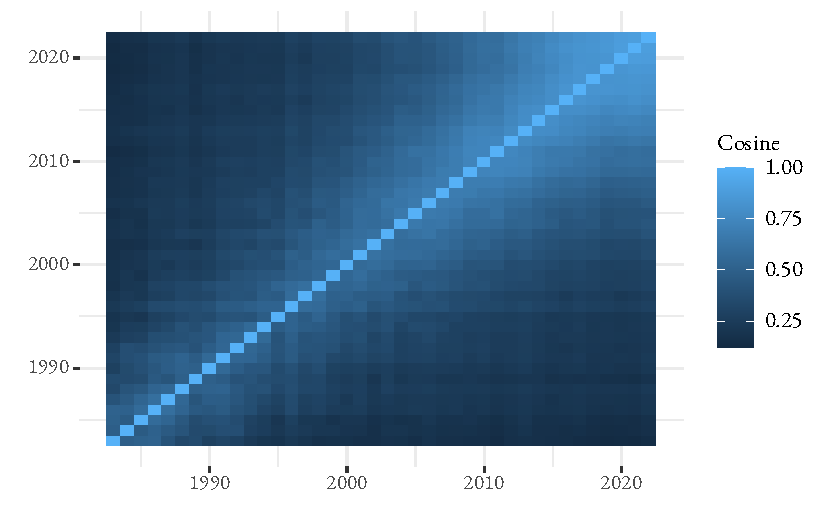
\includegraphics{citation-break_files/figure-pdf/fig-matrix-1.pdf}

}

\caption{\label{fig-matrix}Similarity between citations for different
years.}

\end{figure}%

This starts in 1983 because before that, citations to articles published
1976 or later are few enough that it's mostly just noise.

There doesn't seem to be any sharp break around 2000. To see if I was
missing something, for each year I calculated the average of the
similarity measure between it and the preceding five years, and the
result is Figure~\ref{fig-rolling-average}. Again, I've left out the
very noisy years at the very start; the first year here is 1985, so the
first year whose citations get used is 1980.

\begin{figure}

\centering{

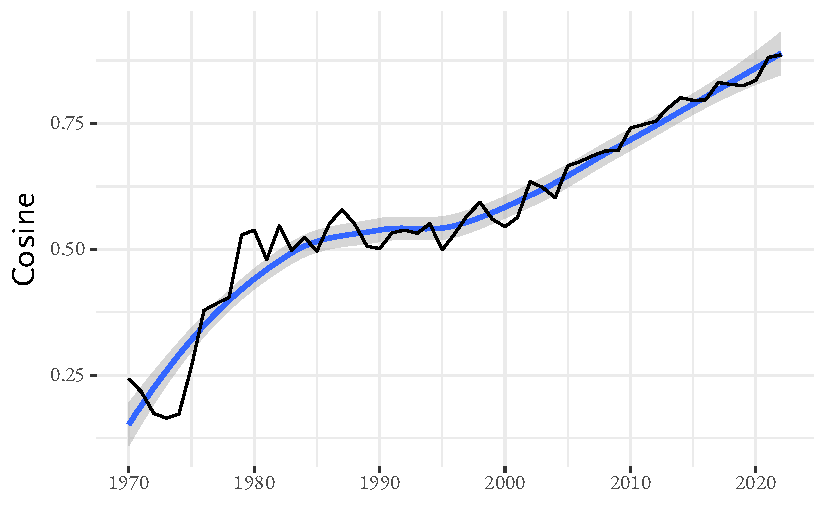
\includegraphics{citation-break_files/figure-pdf/fig-rolling-average-1.pdf}

}

\caption{\label{fig-rolling-average}Similarity between a year's
citations and the previous five years' citations (1985-2022).}

\end{figure}%

The striking thing in Figure~\ref{fig-rolling-average} is how long the
graph takes to start going up. The trend line even goes gently down at
the start. Given the way I've set things up, that shouldn't happen.
Citations tend to go backwards in time, so each year a new hundred
articles are getting added to the range of possible citations. That
makes a small difference at the end; the new articles are only 2\% of
the universe. But it makes a big difference at the start. So graph,
which measures how similar a year is to the previous 5 in how it treats
these 4000 articles, should slope up. Indeed, if we run the exact same
study starting in 1986 rather than 1976, we get
Figure~\ref{fig-rolling-average-late}, which is what I'd a priori
expect.

\begin{figure}

\centering{

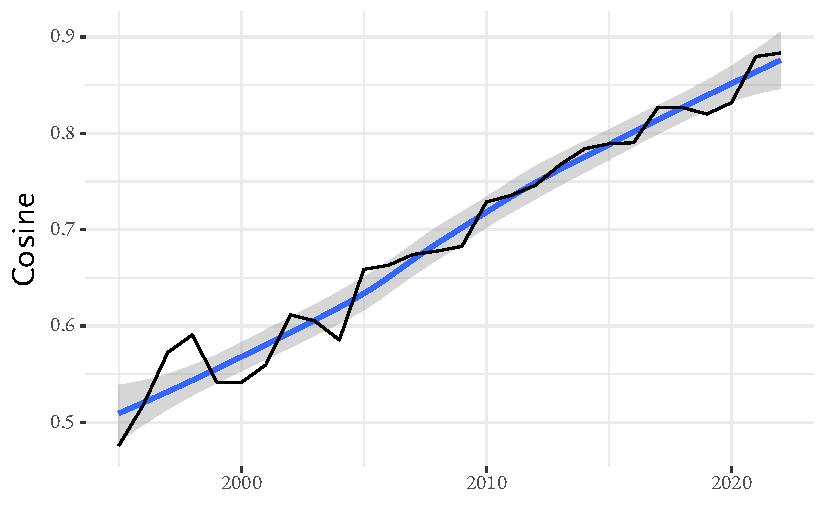
\includegraphics{citation-break_files/figure-pdf/fig-rolling-average-late-1.pdf}

}

\caption{\label{fig-rolling-average-late}Similarity between a year's
citations and the previous five years' citations (1995-2022).}

\end{figure}%

Something odd is happening with the citations to articles from the 1980s
and early 1990s. Here is my conjecture about why we see something like a
break around 2000. There are three things going on at once.

\begin{enumerate}
\def\labelenumi{\arabic{enumi}.}
\tightlist
\item
  Every year there are a huge number of citations to recently published
  papers; lots of replies, and making small moves on top of recent work.
  These kind of citations keep appearing for a decade or more, but they
  gradually fade away.
\item
  Typically, there are a handful of papers that really define a field,
  and while they aren't always immediately recognised as such, they tend
  to keep being cited, in massive volumes, for many years after the
  fact.
\item
  The 1980s saw fewer of these papers being produced, especially after
  1983. So around 2000 the usual turnover of citations, the allure of
  the new, had a more dramatic effect because it wasn't mixed with
  continued discussion of the field defining papers from 10-15 years
  earlier.
\end{enumerate}

Note here that I'm only making a claim about journal articles. There
were some field defining books published in this time, notably \emph{On
the Plurality of Worlds}. And I haven't done a study of chapters in
edited volumes. But the journals stopped producing articles that had
much staying power.

I'll end with a bit more empirical evidence to back this up. Step back
from these 4000 articles and look at all the articles indexed in Web of
Science. For each pair of years x, y, we can ask, for articles published
in year y, what is the mean number of citations they get (in indexed
journals) in year x. The answer is usually pretty low, somewhere between
0.1 and 0.5. For each value of y we get nice little graphs as we vary x.
I'll present these in groups of 5, as well as showing the average value.
So Figure~\ref{fig-mean-most-recent} is what things look like when x is
recent, i.e., 2018-2022.

\begin{figure}

\begin{minipage}{0.50\linewidth}

\centering{

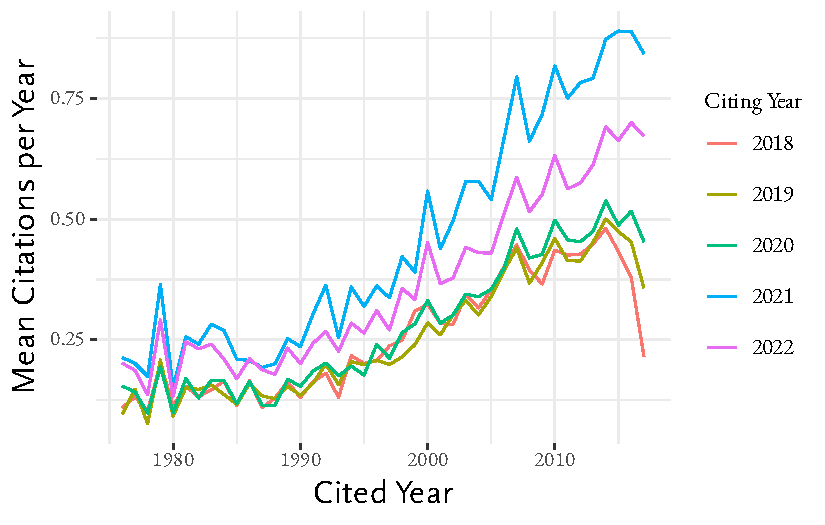
\includegraphics{citation-break_files/figure-pdf/fig-mean-most-recent-1.pdf}

}

\subcaption{\label{fig-mean-most-recent-1}Individual Years}

\end{minipage}%
%
\begin{minipage}{0.50\linewidth}

\centering{

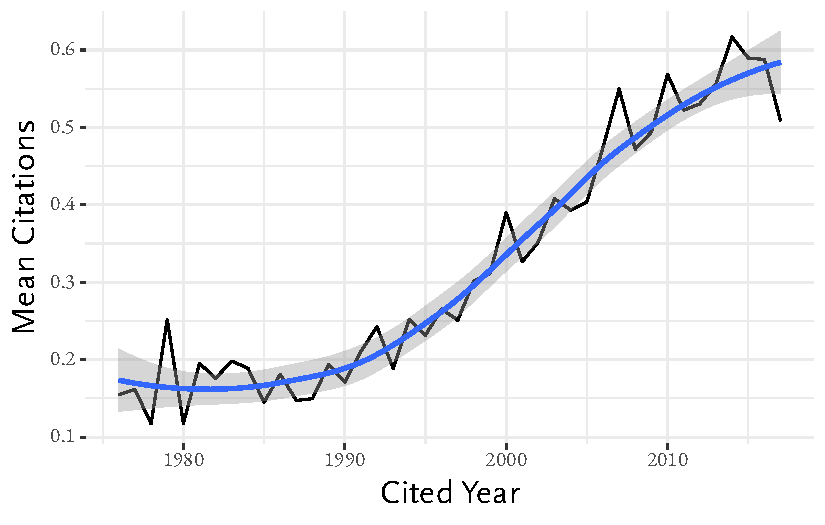
\includegraphics{citation-break_files/figure-pdf/fig-mean-most-recent-2.pdf}

}

\subcaption{\label{fig-mean-most-recent-2}Overall average (2018-2022)}

\end{minipage}%

\caption{\label{fig-mean-most-recent}Mean citations, in 2018-2022, of
articles originally published in different years}

\end{figure}%

There really aren't many citations to articles from the 1980s. But you
might think it was a long time ago, maybe that's just the passage of
time. So let's shift back twenty years earlier, and look (in
Figure~\ref{fig-mean-turn-century}) at what was being cited from
1998-2002, which has been the focus throughout here.

\begin{figure}

\begin{minipage}{0.50\linewidth}

\centering{

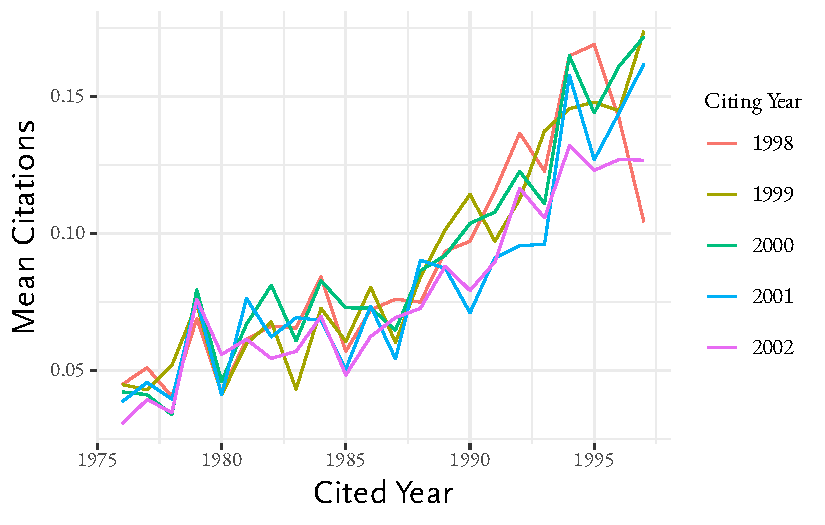
\includegraphics{citation-break_files/figure-pdf/fig-mean-turn-century-1.pdf}

}

\subcaption{\label{fig-mean-turn-century-1}Individual Years}

\end{minipage}%
%
\begin{minipage}{0.50\linewidth}

\centering{

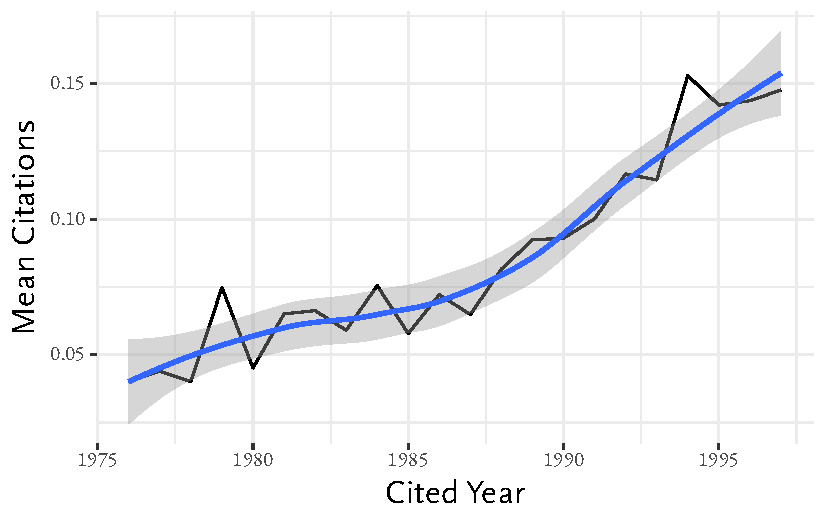
\includegraphics{citation-break_files/figure-pdf/fig-mean-turn-century-2.pdf}

}

\subcaption{\label{fig-mean-turn-century-2}Overall average (1998-2002)}

\end{minipage}%

\caption{\label{fig-mean-turn-century}Mean citations, in 1998-2002, of
articles originally published in different years}

\end{figure}%

Again, there are many fewer citations to articles before about 1991 than
to afterwards. Again, that could just be an age effect, but let's end
with looking at what happened immediately before that, in
Figure~\ref{fig-mean-before-turn}.

\begin{figure}

\begin{minipage}{0.50\linewidth}

\centering{

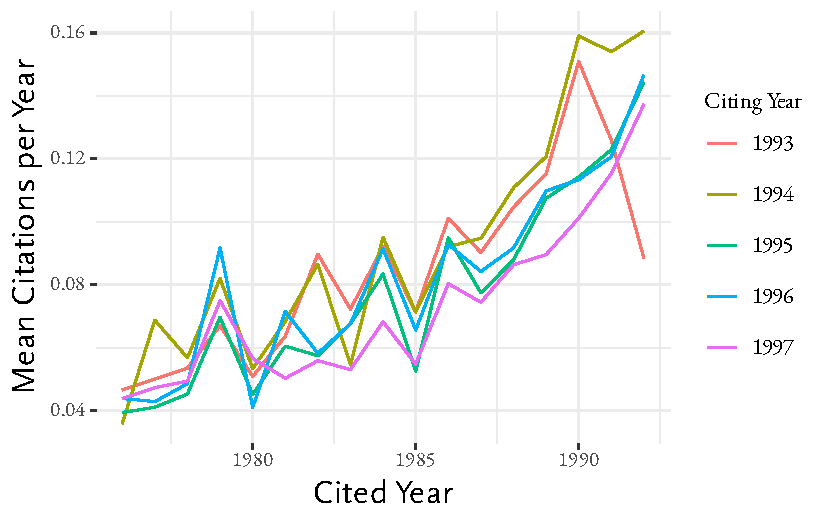
\includegraphics{citation-break_files/figure-pdf/fig-mean-before-turn-1.pdf}

}

\subcaption{\label{fig-mean-before-turn-1}Individual Years}

\end{minipage}%
%
\begin{minipage}{0.50\linewidth}

\centering{

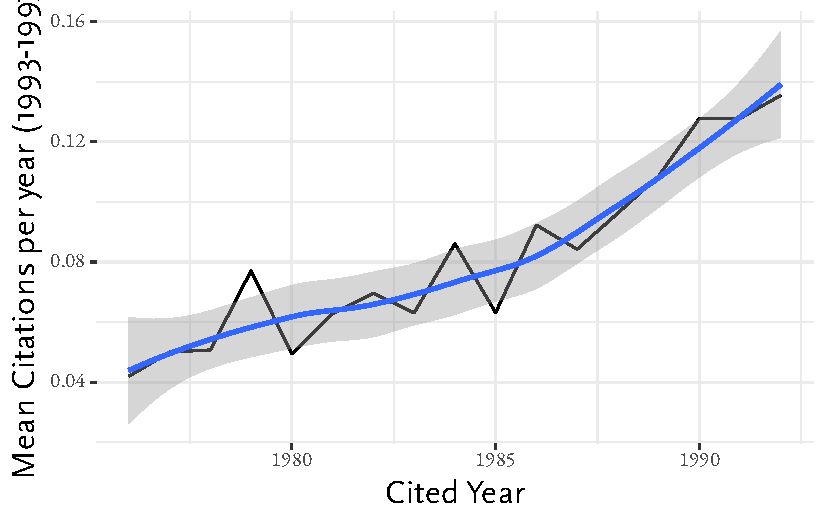
\includegraphics{citation-break_files/figure-pdf/fig-mean-before-turn-2.pdf}

}

\subcaption{\label{fig-mean-before-turn-2}Overall average (1993-1997)}

\end{minipage}%

\caption{\label{fig-mean-before-turn}Mean citations, in 1993-1997, of
articles originally published in different years}

\end{figure}%

In all these graphs there is a recency bias, an upward tick as we get
towards the end. But in Figure~\ref{fig-mean-before-turn} that upwards
bend comes really late. Articles from the 1980s on the whole just
weren't sticking around. Now as I said earlier, I'm only looking at
journals, and for all I've said here, this data just shows that
journals, having become more central in the 1970s, retreated in
importance a little in the 1980s. Or maybe the 1980s had less influence
on philosophy than decades typically do. If so, that would explain the
clustering that Eugenio finds.

So I'll end where I started by saying how grateful I am to the
organisers for putting this on, and to Eugenio for the book. What I've
done here is look at a few things inspired by one section of the book -
it is full of so many insights and observations and it both makes you
rethink what you thought about recent philosophy, and raises many
fascinating questions like the one I've been discussing. I hope it gets
very widely read.

\section*{References}\label{references}
\addcontentsline{toc}{section}{References}

\phantomsection\label{refs}
\begin{CSLReferences}{1}{0}
\bibitem[\citeproctext]{ref-Joyce1998}
Joyce, James M. 1998. {``A Non-Pragmatic Vindication of Probabilism.''}
\emph{Philosophy of Science} 65 (4): 575--603. doi:
\href{https://doi.org/10.1086/392661}{10.1086/392661}.

\bibitem[\citeproctext]{ref-Petrovich2024}
Petrovich, Eugenio. 2024. \emph{A Quantitative Portrait of Analytic
Philosophy: Looking Through the Margins}. Cham: Springer.

\bibitem[\citeproctext]{ref-Williamson1998}
Williamson, Timothy. 1998. {``Conditionalizing on Knowledge.''}
\emph{The British Journal for the Philosophy of Science} 49 (1):
89--121. doi:
\href{https://doi.org/10.1093/bjps/49.1.89}{10.1093/bjps/49.1.89}.

\end{CSLReferences}



\noindent Published online in June 2024.

\end{document}
